\documentclass[12pt,a4paper]{article}

\usepackage[utf8x]{inputenc}
\usepackage[spanish]{babel}
\usepackage{amsmath}
\usepackage{amsfonts}
\usepackage{amssymb}
\usepackage{makeidx}
\usepackage{graphicx}
\usepackage[left=2cm,right=2cm,top=2cm,bottom=2cm]{geometry}

\author{Reyes Alvarez Ulises Isaac\\Cervantes Martinez Luis Osvaldo\\Carrera: Ing. Mecatrónica\\4.B\\Profe. Moran Garabito Carlos Enrique\\Sistemas electrónicos de interfaz\\\\ Universidad Politécnica de la Zona Metropolitana de Guadalajara}

\title{Circuitos de rectificación no controlados}
\date{20/09/2019}

\begin{document}
\maketitle
\begin{figure}[hbtp]
\centering

\includegraphics[scale=1]{UPZMG.png}
\end{figure}

\section*{Objetivos:}
Controlar valores medios de tensión de salida del rectificador mediante ondas\\\\
Identificar los diferentes tipo de rectificadores del convertidor AC-DC

\newpage
\section{Rectificador de media onda con carga inductiva}
\begin{figure}[hbtp]
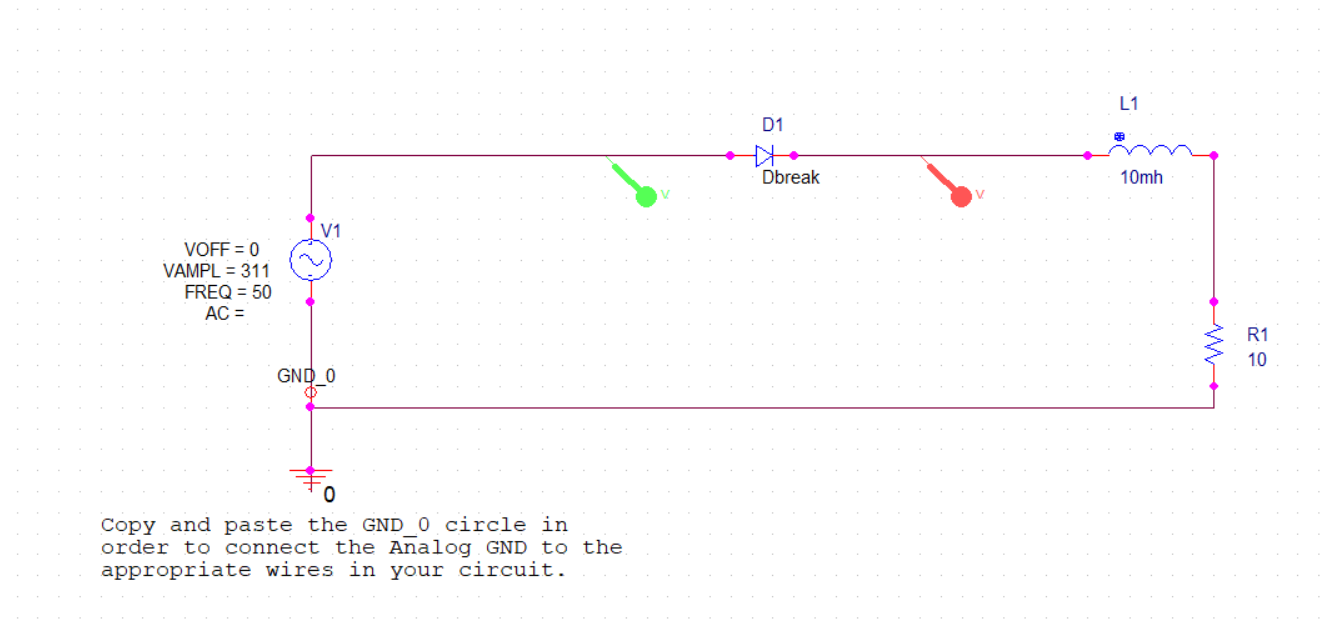
\includegraphics[scale=0.5]{1.png}
\caption{Rectificador de media onda con carga RL}
\end{figure}
Para este circuito utilizamos una fuente(Vsin) con amplitud 311V y con una frecuencia de 50Hz, un diodo (Dbreak), un inductor (L),una resistencia  (R) y la tierra que al agregar una página nueva automáticamente se inserta la tierra, utilizando el simulador OrCAD. \\
Teniendo en cuenta que debemos conectar muy bien los cables para unir los componentes ya que si no es así saldrá error en la simulación.\\
Colocamos dos puntas en el diodo para ver como se comporta la señal y nos aparecerá la señal senoidal.

\begin{figure}[hbtp]
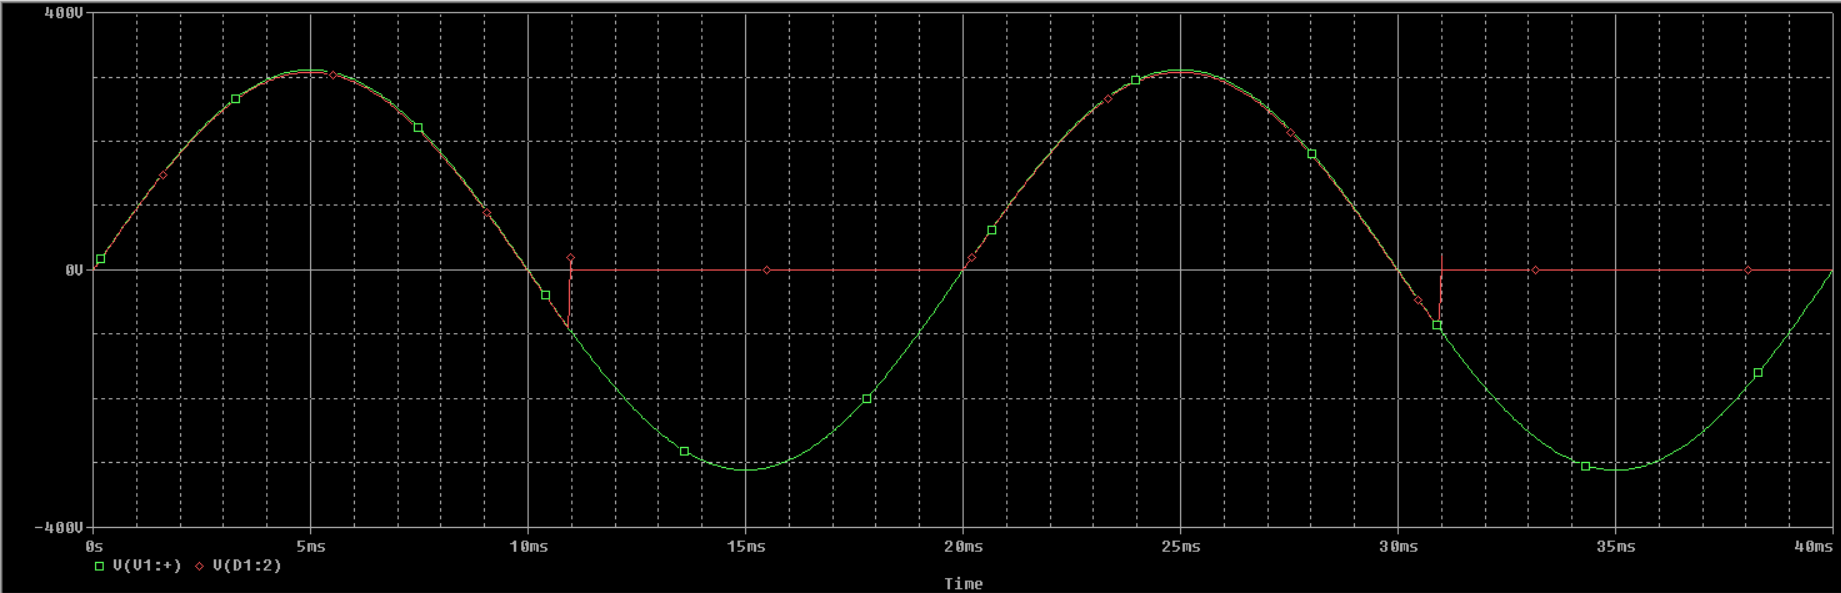
\includegraphics[scale=0.35]{2.png}
\caption{Tensiones de entrada y salida del rectificador}
\end{figure}
Al simular el circuito se puede observar que la onda que se produce, tiene una tensión de salida continua esto hasta que sufre interferencia con la corriente de carga, sufriendo una baja de voltaje, anulándose la corriente, volviendo a repetir se una y otra vez.
Con esto nos podemos percatar de que el diodo tiene una polarización directa, lo cual sería un poco lógico ya que para conectar el ánodo del diodo al polo positivo de la batería y por ende el cátodo al polo negativo, esto genera una polarización directa. Que fue lo que se hizo en nuestro circuito. 

\newpage
\begin{figure}[hbtp]
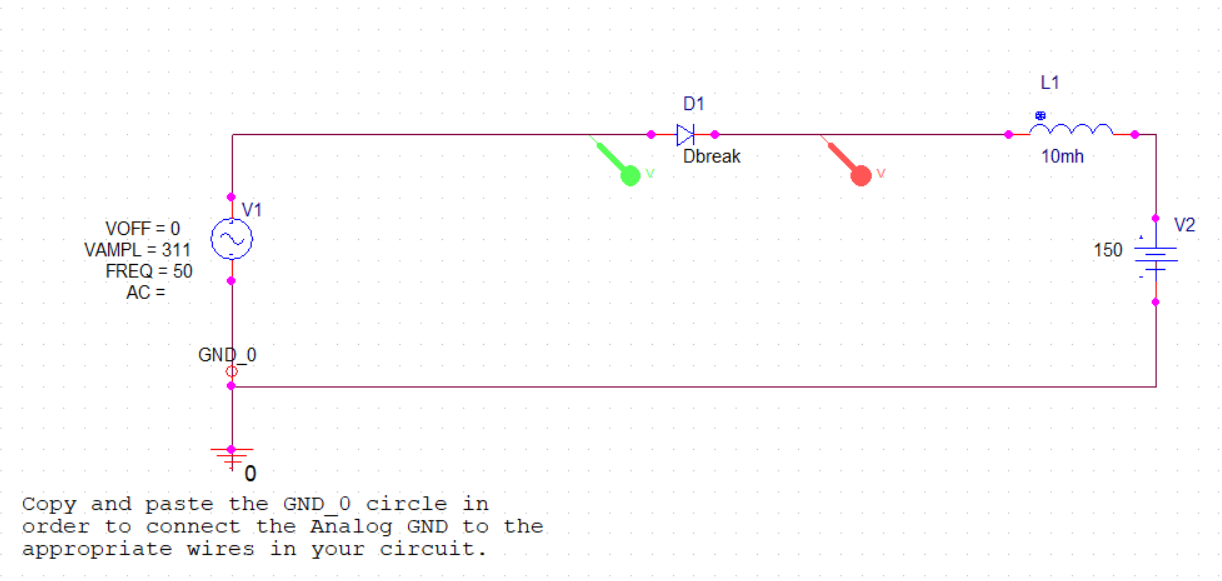
\includegraphics[scale=0.5]{3.png}
\caption{Rectificador de media onda}
\end{figure}
Sustituimos la resistencia por una fuente de corriente continua de valor 150V. Quedando el rectificador monofásico en puente y colocando las dos puntas en el diodo (Dbreak). 

\begin{figure}[hbtp]
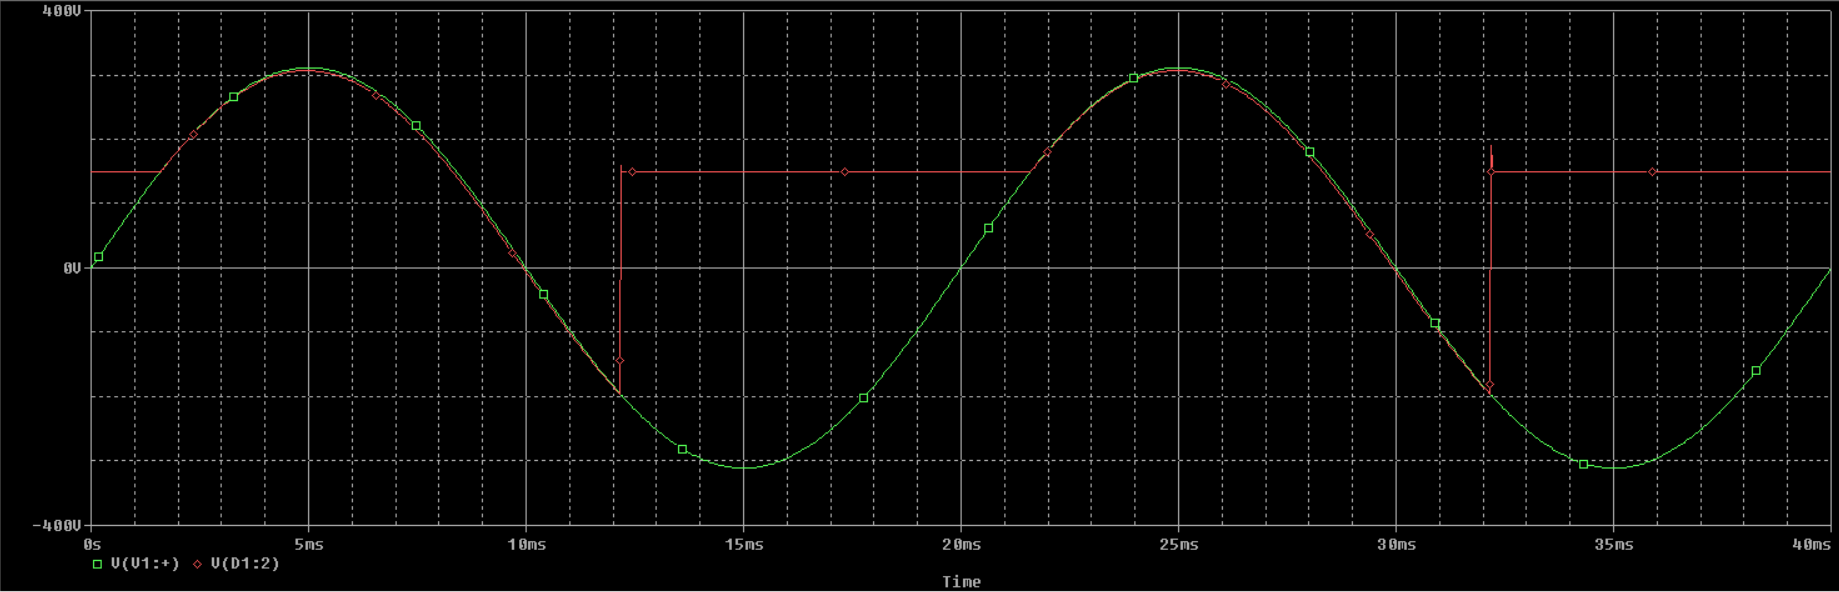
\includegraphics[scale=0.35]{4.png}
\caption{Rectificador de media onda}
\end{figure}
Observamos que en este circuito a diferencia que el anterior, como le hemos modificado nada mas la resistencia por una fuente de corriente continua, observamos que la onda de color rojo empieza mas arriba que la otra y quedando nula en la misma. 

\newpage
\section{Rectificador monofásico en puente}
\begin{figure}[hbtp]
\centering
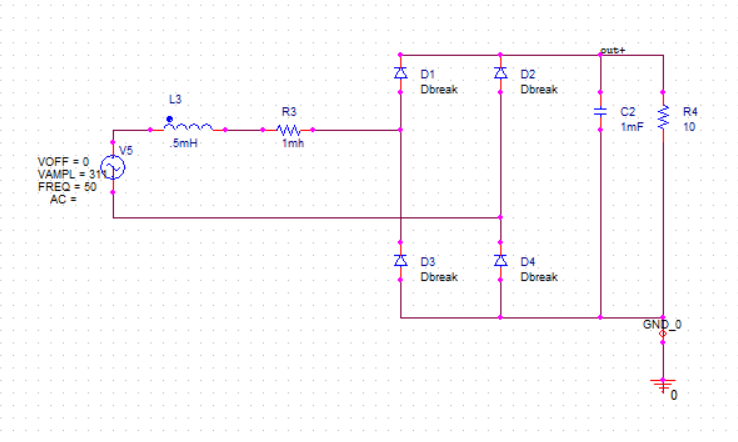
\includegraphics[scale=0.7]{5.png}
\caption{Rectificador monofásico en puente}
\end{figure}
Realizamos el siguiente circuito utilizando los mismos componente de los anteriores circuitos, únicamente agregando un capacitor (C), los demás componentes ya sabemos como se llaman y pasamos a armarlo. 

\begin{figure}[hbtp]
\centering
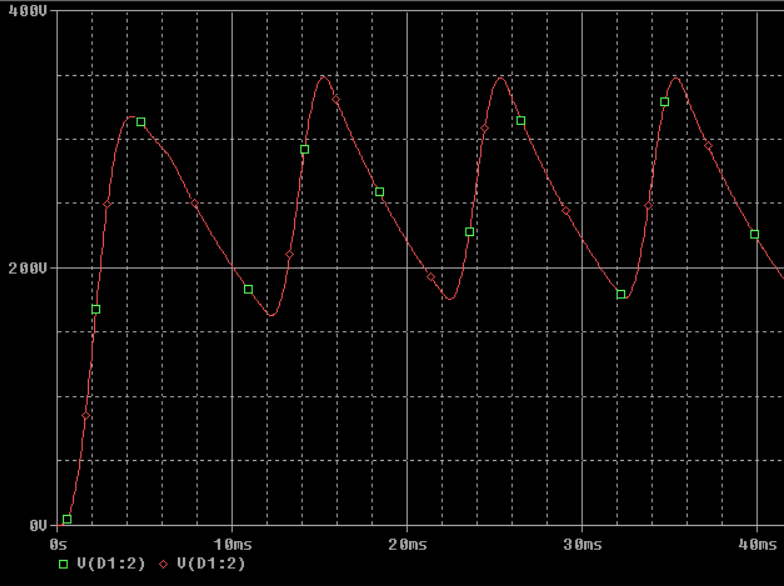
\includegraphics[scale=0.5]{6.png}
\caption{Tensión salida del rectificador}
\end{figure}
La simulación de este circuito no es más, que el proporcionarnos un análisis de Fourier, el cual en esta ocasión se genera con la corriente que concede la entrada del rectificador.
El análisis de Fourier no es más que un estudio de representaciones de señales como superposición de ondas básicas o armónicos.

\newpage
\section{Rectificador monofásico duplicador de tensión}
\begin{figure}[hbtp]
\centering
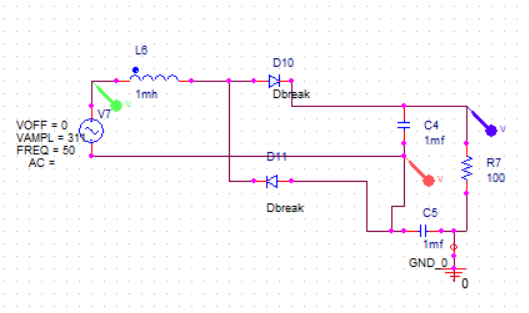
\includegraphics[scale=0.8]{7.png}
\caption{Rectificador duplicador de tensión}
\end{figure}
Realizamos el siguiente circuito en el simulador, ocupando los mismos componentes de los circuitos anteriores,con una amplitud en la fuente de 311V, con 60Hz de frecuencia, y colocando las puntas en el antes del inductor, otra después del capacitor y una ultima entre el capacitor anterior y la resistencia en paralelo.

\begin{figure}[hbtp]
\centering
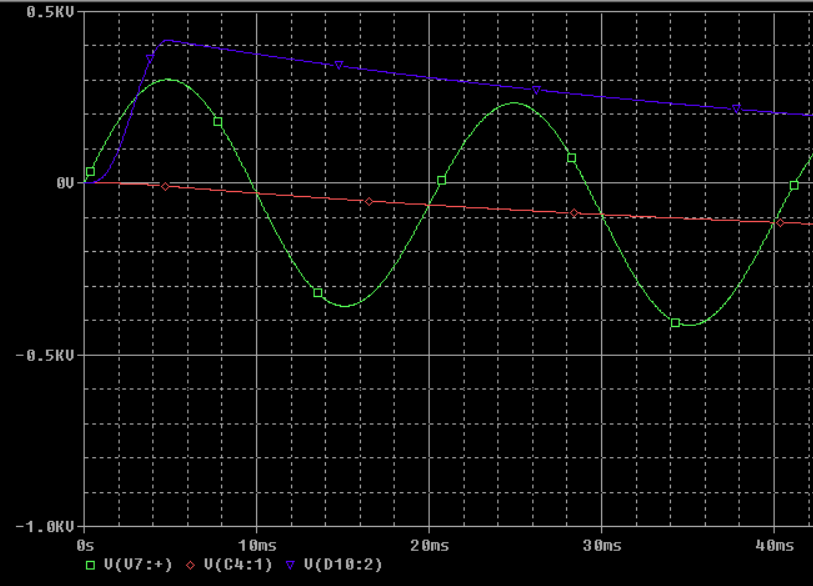
\includegraphics[scale=0.45]{8.png}
\caption{Rectificador de media onda}
\end{figure}
En este circuito se vuele a generar un rectificador, el cual al simularlo nos muestra la apariencia que tiene la onda de tensión de salida de éste. El cual podemos observar por medio de la onda generada por el color azul.

\newpage
\section{Efectos de los rectificadores monofásicas en líneas trifásicas}
\begin{figure}[hbtp]
\centering
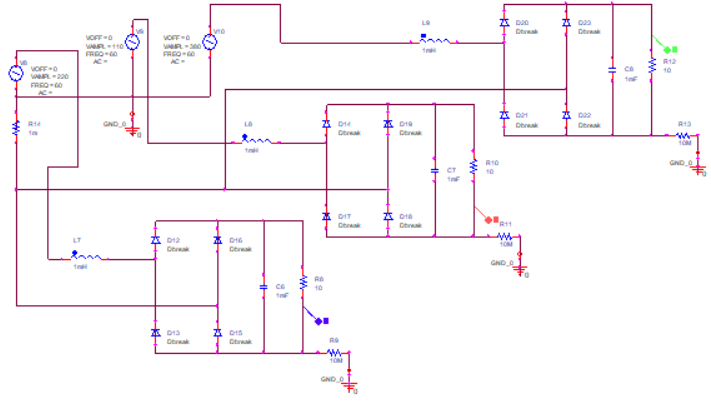
\includegraphics[scale=0.7]{9.png}
\caption{Esquema de conexión de tres rectificadores monofásicos a una línea a 4 hilos}
\end{figure}
Para la realización de este proyecto tuvimos que realizar 3 subcircuitos del rectificador monofásico y conectarlos en paralelo y en serie con las fuentes, dándole valores a cada una de las fuentes, la primera de amplitud 380V, con 60Hz, la segunda con amplitud 110V con 60Hz, y la tercera con amplitud 220V con 60Hz.\\
Colocando las puntas en la ultima resistencia, en el primer circuito arriba de la resistencia y las otra dos debajo de las resistencias.

\begin{figure}[hbtp]
\centering
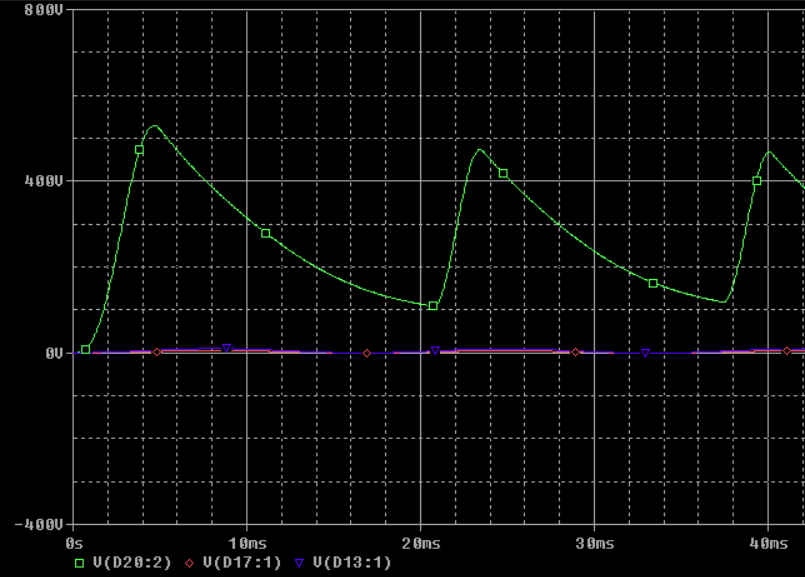
\includegraphics[scale=0.45]{10.png}
\caption{Corriente en uno de los conductores de línea }
\end{figure}
En este circuito se ilustra una instalación conformada por tres receptores mofasticos de iguales características y un neutro. El cual al simular genera una onda como la de color verde mostrada en la imagen. 

\newpage
\section{Rectificadores trifásicos}
\begin{figure}[hbtp]
\centering
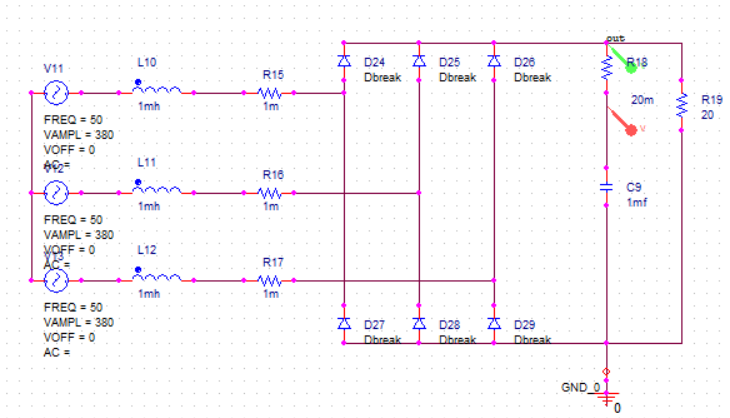
\includegraphics[scale=0.5]{11.png}
\caption{Esquema del rectificador trifásico no controlado}
\end{figure}
Con el siguiente circuito obtendremos el comportamiento de la onda senoidal teniendo 3 inductores, colocando nuestras puntas en la ultima resistencia, teniendo en nuestra fuente 380V de amplitud con 60Hz de frecuencia.

\begin{figure}[hbtp]
\centering
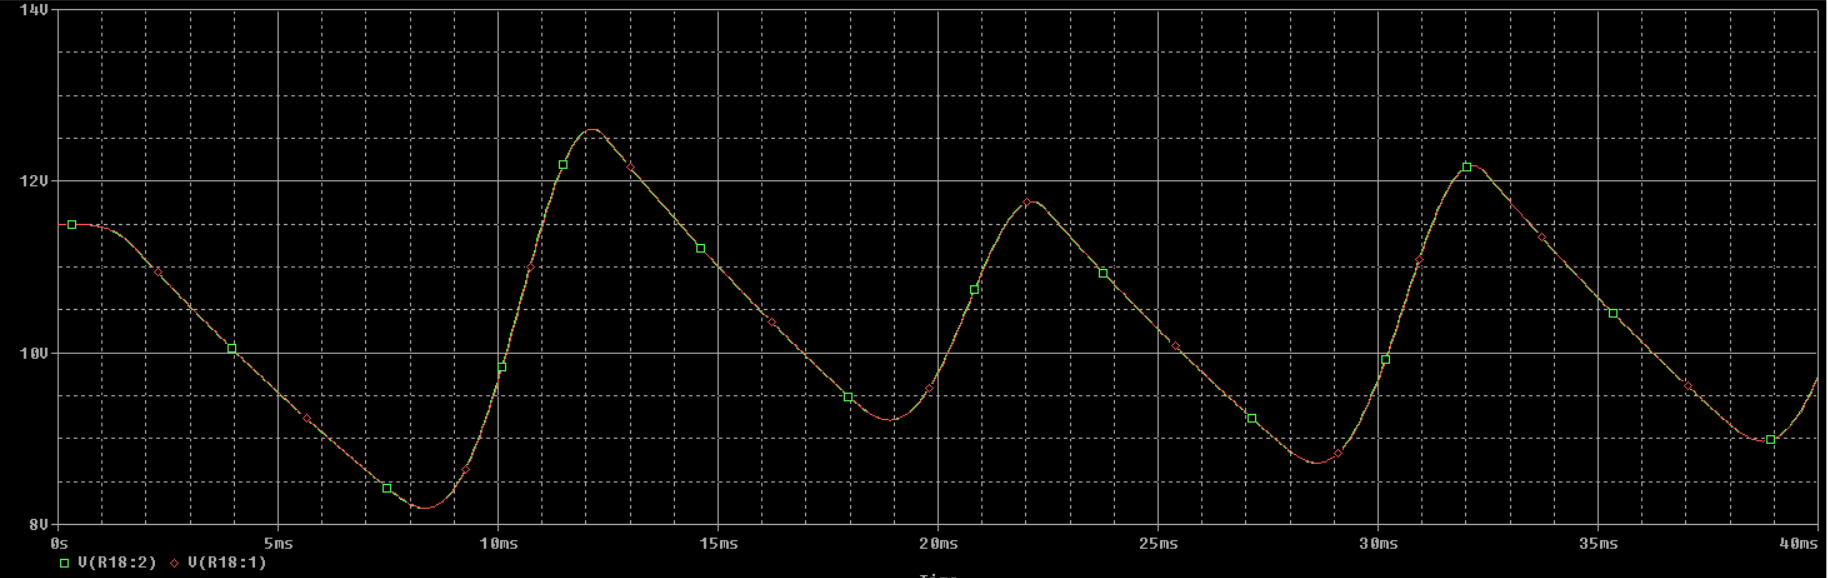
\includegraphics[scale=0.35]{12.png}
\caption{Tensión de salida del rectificador}
\end{figure}
Para simular este circuito fue necesario desfasar las tres resistencias del circuito ya que de no ser así esto provocaba que las tensiones chocaran lo que puede aparentar una onda muerta. Al desfasarlos se puede observar los desequilibrios de las fases, proporcionado por la intensidad de entrada, generando una onda no armónica.

\newpage
\section{Efecto de las inductancias de red sobre la conmutación de corriente}
\begin{figure}[hbtp]
\centering
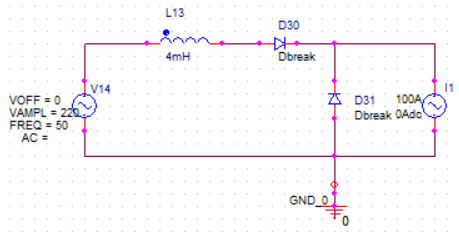
\includegraphics[scale=0.9]{13.png}
\caption{Circuito básico de conmutación entre diodos}
\end{figure}
Para el siguiente circuito ocupamos una fuente con 220V de amplitud, 50Hz de frecuencia, el inductor de 4mH, dos diodos y por ultimo una fuente de corriente con 100A.
Colocando las puntas entre los diodos para ver el efecto de conmutación. 

\begin{figure}[hbtp]
\centering
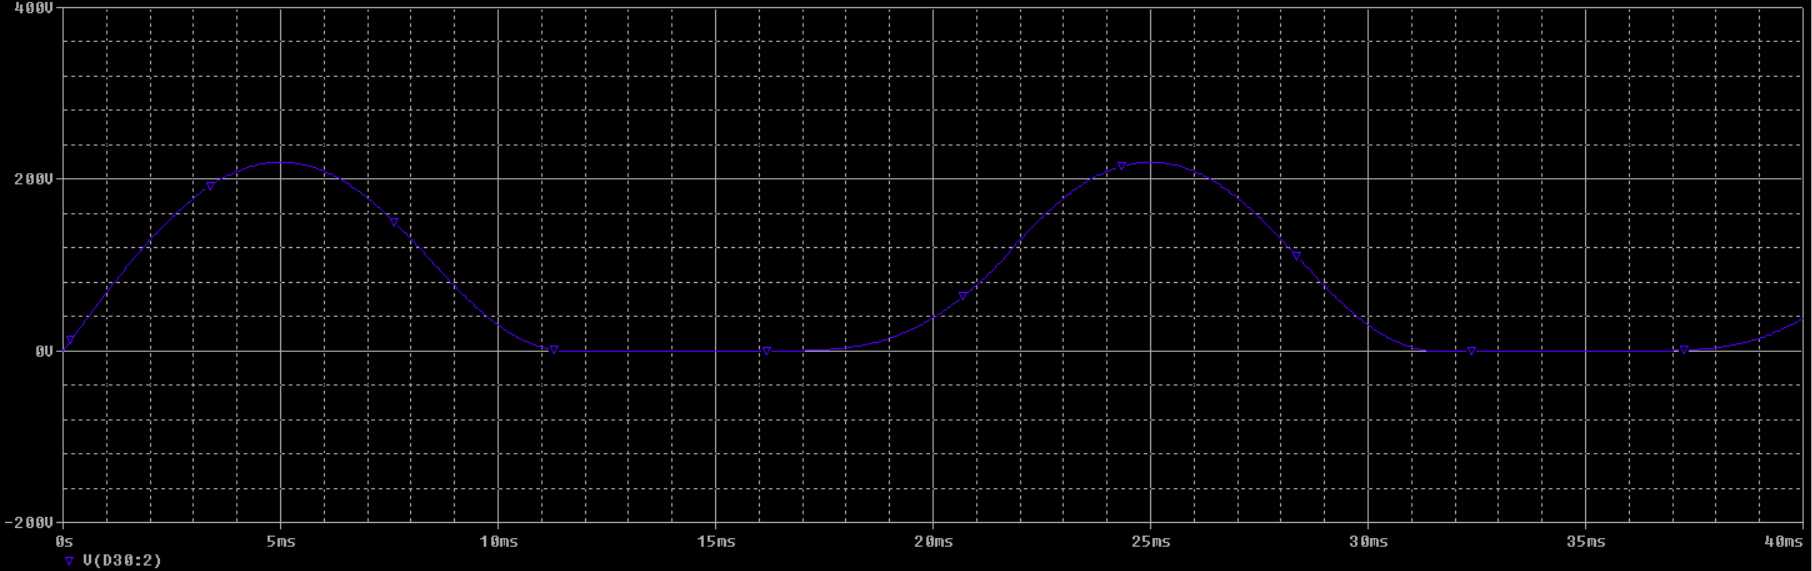
\includegraphics[scale=0.35]{14.png}
\caption{Tensión de salida cuando la conmutación de los diodos es prácticamente instantánea}
\end{figure}
La onda generada por este circuito se debe de la falta de inductancias, que es una fuerza proporcionada por la variación del paso de corriente, lo cual genera que durante la conducción del segundo diodo sea casi nula y prácticamente la de entrada seria durante la conducción del primer diodo. Lo cual se refleja en la onda que se puede observar en la simulación. 

\newpage
\section*{Conclusiones}
\section*{Cervantes Martinez Luis Osvaldo}
Para la conversión de la corriente alterna a corriente continua se necesitan dos tipos de convertidores:
1.Rectificadores controlados 
2.Rectificadores no controlados
Que ayudan a dejar pasar la onda senoidal en un solo voltaje pico mediante diodos (rectificador no controlado) o por tiristores (rectificador controlado), creando la corriente directa con el cual muchos dispositivos electrónicos ocupan de esta corriente para funcionar mejor.

\section*{Reyes Alvarez Ulises Isaac}
Algunos receptores electrónicos requieren de corriente directa para su correcto funcionamiento, requiriendo una red eléctrica que es utilizada como fuente de suministro de energía y con ello utilizando circuitos rectificadores encargados de transformar en continuas las formas de las ondas alternas. Sabiendo que existen dos tipos de convertidores: no controlados y controlados.
Los rectificadores no controlados utilizan diodos como dispositivo semiconductor y permiten obtener una tensión de salida con un valor medio contante, se dice que es el más utilizado por su simplicidad.
Y los rectificadores controlados que utilizan tiristores como dispositivo semiconductor. 

\end{document}